\section{Propuesta de Solución}

\subsection{Preprocesamiento e Ingeniería de Características}
Debido al origen natural del gasto humano, caracterizado por una fuerte estacionalidad a lo largo del año y por patrones repetitivitos inherentes, diseñamos un marco de preprocesamiento robusto previo al entrenamiento de cualquier modelo algorítmico, cuyos detalles se listan a continuación:
\begin{itemize}
    \item \textbf{Agrupación y Limpieza General}: Eliminación de caracteres simbólicos (\textit{€}), interpolación de datos inconsistentes (NaT) originados en la columna `Amount` por lecturas imprecisas e indexación de la serie en rangos diarios para la uniformidad de la base.
    \item \textbf{Factores de Estacionalidad y Componentes de Tiempo}: Creación de los predictores clave que engloban \textit{Quarter} (Trimestre), \textit{Mes}, variaciones asociadas al verano (\textit{Is\_Summer}) e indicativos del mes principal de dispendio humano (\textit{Is\_December}). Estas variables dotan a cualquier árbol de decisión de contexto.
    \item \textbf{Generación de Variables Retardadas (Lags)}: Los hábitos humanos son autoregresivos. Se han incluido los gastos y ganancias de hace varios horizontes espaciales: concretamente $1, 2, 3$ y $12$ meses de retrospectiva (\textit{Lag 1, 2, 3, 12}), sirviendo como principal insumo predictor de comportamiento cíclico interanual e intra-trimestral de modo que el modelo evalúa qué ocurrió el mismo mes del año anterior.
    \item \textbf{Medias Móviles (Rolling Statistics)}: Complementando a los Lags, calculamos una ventana rodante (sobre medias exponenciales EMA3 y ventana natural a 3 y 6 meses). Actúa como factor de suavizado, estabilizando las posibles disrupciones atípicas para proveer un vector firme de predicción para la tendencia actual económica.
\end{itemize}

\subsection{Modelos de Análisis y Predicción Implementados}
El entrenamiento de esta solución se basó en una experimentación comparativa abordando:
\begin{enumerate}
    \item \textbf{Linear Regression (Baseline)}: Como punto de partida de referencia para certificar las posteriores ganancias de información.
    \item \textbf{XGBoost, Random Forest e HistGradientBoosting}: Familia de métodos de ensamblado basados en árboles de decisión, que actúan de manera estelar resolviendo las relaciones no-lineales subyacentes presentes en la lógica de las características estacionales \textit{One-Hot} y los lags retardados.
    \item \textbf{ARIMA y SARIMAX}: Alternativas analítico-estadísticas clásicas focalizadas exclusivamente en la regresión temporal intrínseca frente al historial de observaciones directas y la autocorrelación de sus rezagos sin tantas características contextuales combinadas.
    \item \textbf{Voting Regressor (Ensemble final)}: Combinación agregativa orientada específicamente a disminuir la sensibilidad a la varianza y estabilizar la predicción sobre aquellos modelos ensamble con los índices absolutos de error (MAE) más eficientes.
    \item \textbf{Recurrent Neural Network (LSTM)}: Un enfoque profundo para encontrar memoria secuencias a largo/corto plazo sobre las capas recursivas ajustadas por épocas de validación cruzada.
\end{enumerate}

Para sustentar documentalmente la evolución algorítmica y su comportamiento durante el entrenamiento o en el ciclo final de test, se añaden a continuación las pertinentes capturas procedentes de la ejecución final del estudio:

% [INSTRUCCIÓN_PARA_EL_USUARIO: Insertar aquí capturas del código de preprocesamiento de características y/o gráficas de evaluación comparativa generadas con `plot_actual_vs_predicted_multiple`]
\subsection{Análisis de Resultados y Validación}

Tras la implementación de los modelos descritos, se procedió a una validación experimental para contrastar su desempeño bajo distintas condiciones de datos, permitiendo justificar la elección del modelo final.

En la Figura \ref{fig:comparation_orig}, se presenta la comparativa inicial utilizando el dataset bruto. El resultado evidencia la ineficacia de la Regresión Lineal ante datos con alta varianza y presencia de valores atípicos, presentando un error (MAE) que triplica al de los modelos de ensamble. Esto ratifica que la relación entre las características temporales y el gasto no es lineal.

\begin{figure}[h]
    \centering
    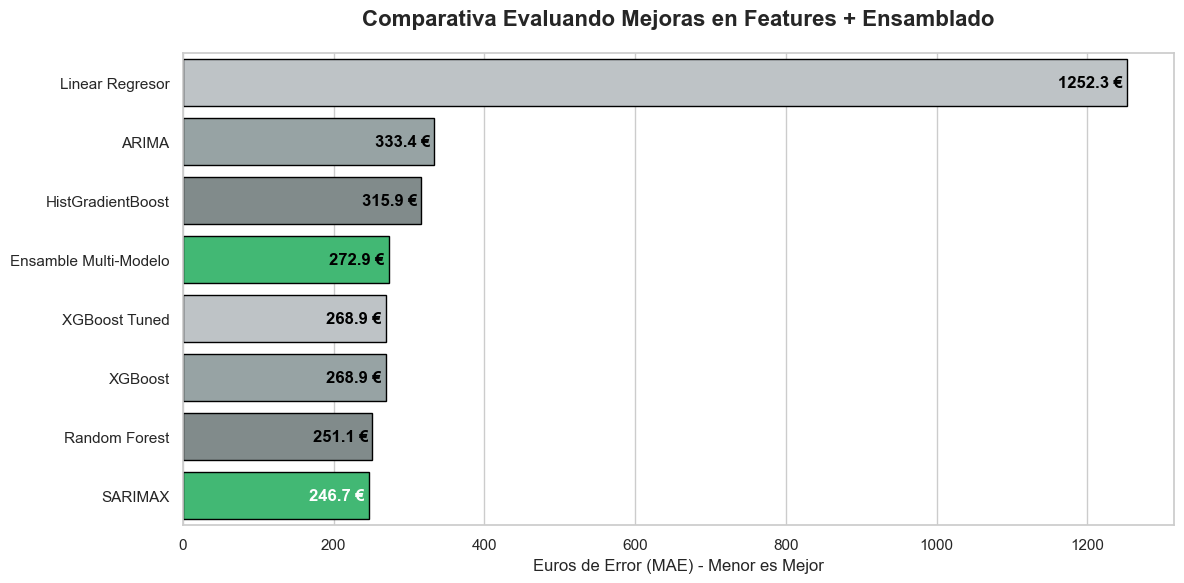
\includegraphics[width=0.85\textwidth]{comparation_orig.png}
    \caption{Evaluación del MAE con datos originales: se observa la vulnerabilidad del modelo lineal frente a la robustez de los algoritmos de árboles.}
    \label{fig:comparation_orig}
\end{figure}

Posteriormente, se realizó un truncado de valores atípicos a 8.000 \texteuro{} para evaluar la sensibilidad al ruido. Como muestra la Figura \ref{fig:comparation_8779}, si bien esta limpieza reduce drásticamente el error del modelo base (LR), los modelos de \textit{Random Forest} y \textit{Boosting} mantienen su superioridad. Esto demuestra que su capacidad predictiva no depende solo de la ausencia de valores extremos, sino de la captura de patrones cíclicos mediante los \textit{lags} generados[cite: 4, 13].

\begin{figure}[h]
    \centering
    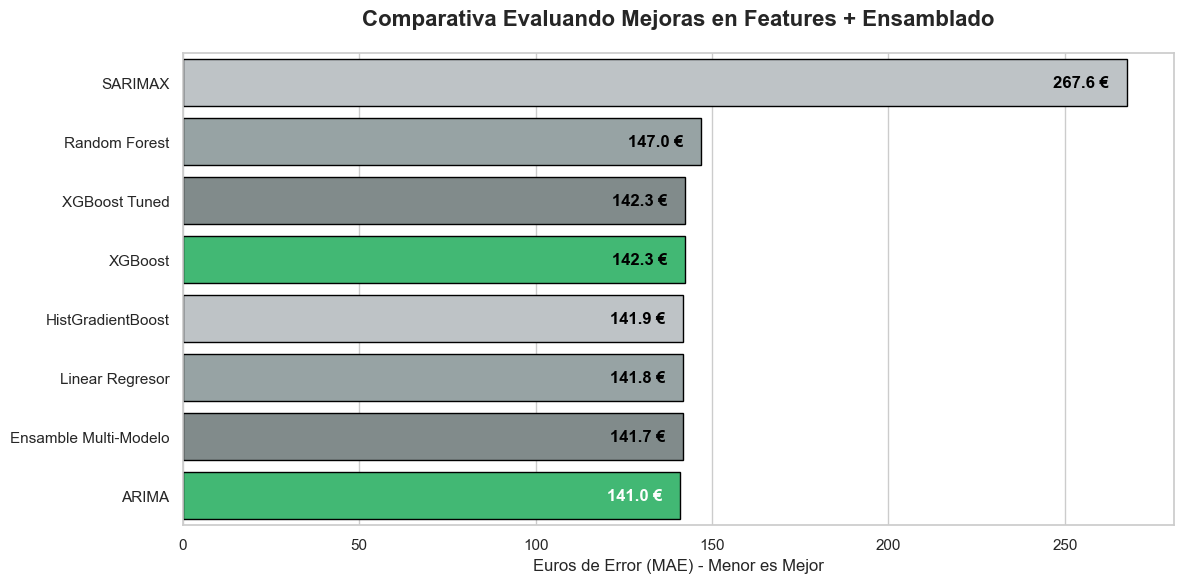
\includegraphics[width=0.85\textwidth]{comparation_8779.png}
    \caption{Impacto del truncado de datos a 8.000 \texteuro{}: mejora de la convergencia en modelos simples y consolidación de los modelos de ensamble.}
    \label{fig:comparation_8779}
\end{figure}

\subsection{Selección del Modelo y Desempeño del MVP}

Finalmente, se seleccionó el modelo \textbf{Random Forest} debido a su estabilidad y precisión consistente en ambas pruebas. La Figura \ref{fig:resultado_final_rf} ilustra el desempeño final en el conjunto de test, donde la línea de predicción captura con éxito la estacionalidad y las fluctuaciones del gasto real[cite: 15]. Este resultado visual confirma que la estrategia de preprocesamiento y el algoritmo seleccionado son capaces de anticipar con éxito el comportamiento económico del usuario.

\begin{figure}[h]
    \centering
    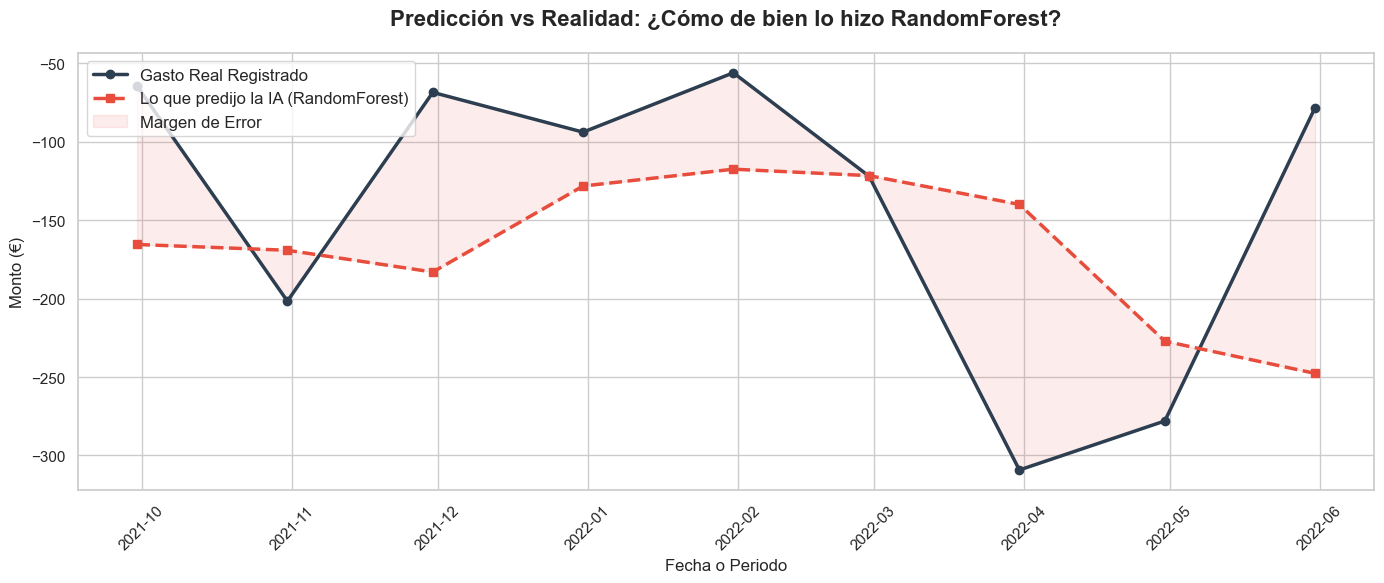
\includegraphics[width=0.95\textwidth]{orig_RandomForest_actual_vs_predicted.png}
    \caption{Contraste entre valores reales y predicción final del MVP (Random Forest). Se observa una alta correlación en la tendencia temporal[cite: 15].}
    \label{fig:resultado_final_rf}
\end{figure}